\documentclass{beamer}

\title{Small Aggregates, Big Manipulation: Vote Buying Enforcement and Collective Monitoring}
\subtitle{A Replication Exercise}
\author{Haseeb Bajwa, Rithika Kumar, John Matthews}

%\usetheme{lucid}
\begin{document}
	\frame {
		\titlepage
	}
	\frame {
		\frametitle{Summary}
		\begin{itemize}
		    \item Rueda looks at the incentives and conditions under which parties ensure compliance of voters in Colombia
		    \item Specifically, he studies the relationship between polling station size and incidence of vote buying
		    \item Mechanism: Election results of small groups of people make voters feel that their vote can be important in reaching the threshold of votes considered acceptable by brokers to deliver future rewards
		    \item Prediction: Higher disaggregation of voting results helps in sustaining vote buying, despite the fact that brokers are not entirely certain of actual individual voting behavior 
		    \item Fuzzy RDD that uses an arbitrary rule on maximum size of polling stations to exploit the exogenous variation in polling station size
		\end{itemize}
	}
	
	\frame{
	    \frametitle{Data}
	    \begin{itemize}
	        \item Number of citizen's reports from every municipality per election (2002-2011)
	        \item Problem: under-reporting due to resistance to reporting
	        \item Election monitor reports collected by the MOE from 632 municipalities (2006-2011)
	        \item Problem: sample bias due to logistical limitations
	        \item Population size: Registered voters per polling place
	        \item Population size: Population 20+ years old per polling place
	        \item Municipal controls for economic indicators, armed group presence
	    \end{itemize}
	    
	}

\frame{
\frametitle{Replication}
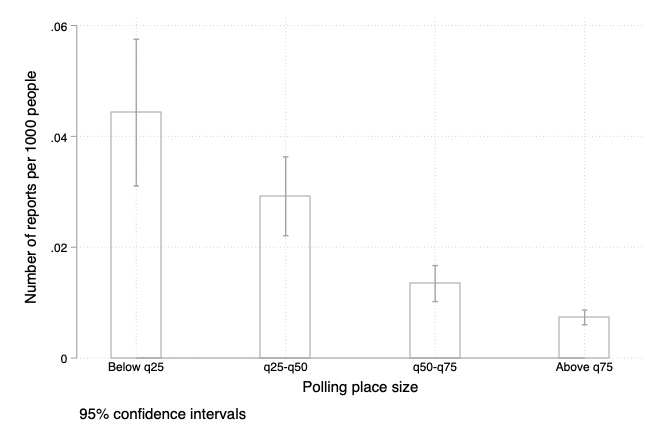
\includegraphics[scale = 0.4]{fig1.jpg}		
}	
	
	\frame{
	\frametitle{Replication}
	\begin{table}[]
    \caption{Simple Replication of Table 2}
    \centering
\scalebox{0.80}{
\begin{tabular}{l*{1}{ccc}}
\hline
                    Dependent Variable &\multicolumn{3}{c}{Citizens' Vote Buying Reports}\\
                   Size Measure &\multicolumn{}{c}{ln(Registered / Stations)}&\multicolumn{2}{c}{ln(Pop. age \geq 20 / Stations)}\\
                    &(1)&(2)&(3)\\
\hline
Polling Place Size&-1.929&-1.544&-1.1158\\
                    &(0.3633)&(0.2321)&(0.2509)\\

Armed Group &&&-0.32402\\
                  &&&(0.1225)\\

Electorate Size&&&-0.3704\\
                    &&&(0.02866)\\

Municipality controls&no&no&yes \\

\hline
Observations        &4473&4473&4352\\
\hline\hline
\multicolumn{2}{l}{\footnotesize \textit{t} statistics in parentheses}\\
\end{tabular}
}
\end{table}
	}

	\frame{\
	\frametitle{Replication}
	\begin{table}[]
    \caption{Simple Replication of Table 3}
    \centering
\scalebox{0.75}{
\begin{tabular}{l*{1}{cccccc}}
\hline
                    Dependent Variable: &\multicolumn{4}{c}{Monitors' Vote Buying Reports}\\
                    \hline
                   &\multicolumn{4}{c}{Original Data}&\multicolumn{2}{c}{Multiple Imputation}\\
                   \hline
                    &(1)&(2)&(3)&(4)&(5)&(6)\\
                    
\hline
Polling Place Size&-1.627&-0.93&-0.963&-4.445&-.4482&-1.383\\%results are in resultsmib.dta in replication folder 
                    &(0.496)&(0.437)&(1.524)&(1.573)&(0.1841)&(0.7899)\\


Municipality controls&no&yes&yes&yes&yes&yes \\
Municipality fixed effect&no&no&yes&yes&no&yes\\
Model &NB&NB&Poisson FE&FE&NB&Poisson FE\\

\hline
Observations        &1075&1069&222&1069&4488&2911.6\\
Municipalities &634&632&82&632&1122&727.9\\
\hline\hline
\multicolumn{4}{l}{\footnotesize \textit{t} statistics in parentheses}\\
\end{tabular}
}
\end{table}
	}

	\frame{
	\frametitle{Replication}
	\begin{table}[]
    \caption{Simple Replication of Table 4}
    \centering
\scalebox{0.80}{
\begin{tabular}{l*{1}{ccc}}
\hline
                    Dependent Variable &\multicolumn{3}{c}{1 if Offered Bribe, 0 Otherwise}\\
                    &(1)&(2)&(3)\\
\hline
Polling Place Size& -0.349 & -0.364 &-3.123\\
                    &(0.168)&(0.168)&(1.181)\\

Cultural individual controls & no & yes & yes \\

Municipality Controls & no & no & yes\\

Municipality Fixed Effects &no&no&yes \\

Model & Logit & Logit & Logit \\

Observations & 3636 &3636&3636\\
Municipalities & 77 & 77 & 77 \\
\hline
\end{tabular}
}
\end{table}
	}

	
	\frame{
		\frametitle{Extension}
		\begin{itemize}
			\item 		In the first part of the extension we present the results (from both tables) separately for national and state level elections. 
			\item Next we drop outlier values of observer reports of vote buying in order to ensure that the results are not being overestimated due to these observations.
			\item Next, we identify the five most populous \textit{departamentos} in Colombia and re-run the analysis on this sub-sample of observations.
		\end{itemize}
	}

	
\frame{
\frametitle{Extension}
\begin{table}[]
    \caption{Extension of Table 2, Column 1 with Controls Added}
    \centering
\scalebox{0.90}{
\begin{tabular}{l*{1}{c}}
\hline
                    &\multicolumn{1}{c}{Vote Buying, Citizens' Reports}\\
\hline
Polling Station Size&      -0.356\\
                    &     (-0.79)\\
Armed Group &      -0.306\\
                  &     (-2.43)\\

Electorate Size&      -0.386\\
                    &    (-13.55)\\

Municipality controls& yes \\

\hline
Observations        &        4352\\
\hline\hline
\multicolumn{2}{l}{\footnotesize \textit{t} statistics in parentheses}\\
\end{tabular}
}
\end{table}
}	

\frame{
\frametitle{Extension}
\begin{table}[]
    \caption{Extension of Table 2 with Subsetting For National and State Elections}
 \singlespacing   
    \centering
{    
\scalebox{0.80}{

\begin{tabular}{l*{1}{cccccc}}
\hline\hline
                    &\multicolumn{3}{c}{\large National Elections}&\multicolumn{3}{c}{\large State Elections}\\
                \hline
                    Dependent Variable &\multicolumn{6}{c}{Citizens' Vote Buying Reports}\\
                    
                   \hline 
                    &(1)&(2)&(3)&(4)&(5)&(6)\\
                \hline    



Polling Place Size&0.924&-1.364&-1.565&-0.202&-1.076&-1.160\\
                    &      (1.15)&(-2.98) & (-3.06)& (-0.48)&(-4.12)&(-4.26)\\
                  
Armed Group&&&       0.269&&&      -0.222\\
                    &&&      (0.93)&&&     (-1.86)\\
Electorate Size&&&      -0.182&&&     -0.0610\\
                    &&&     (-0.02)&&&     (-0.74)\\
Municipality Controls &no&no& yes&no&no&yes\\
\hline  
Observations        &        2236&        2236&        2172&        2237&        2237&        2180\\
\hline\hline
\multicolumn{2}{l}{\footnotesize \textit{t} statistics in parentheses}\\
\end{tabular}}}
\end{table}
}	

\frame{
\frametitle{Extension}
\begin{table}[]
    \caption{Extension of Table 3 with Subsetting For National and State Elections}
 \singlespacing   
    \centering
{    
\scalebox{0.80}{

\begin{tabular}{l*{1}{cccc}}
\hline\hline
                    &\multicolumn{2}{c}{\large National Elections}&\multicolumn{2}{c}{\large State Elections}\\
                  
                    
Dependent Variable: &\multicolumn{4}{c}{\large Vote Buying - Monitors' Reports}\\
  &(1)&(2)&(3)&(4)\\
\hline
Polling station Size 
&-1.538&       27.63&      -0.598&      -3.546\\
&(-1.79)&(6980.76)&     (-1.10)&     (-0.94)\\

Municipality controls&no&yes&no&yes \\
Municipality fixed effect&no&yes&no&yes\\
Model &NB&FE&NB&FE\\

\hline
Observations        &295&         295&         780&         774\\
\hline\hline
\multicolumn{2}{l}{\footnotesize \textit{t} statistics in parentheses}\\
\end{tabular}}}
\end{table}
}

\frame{
\frametitle{Extension}
\begin{table}[]
    \caption{Extension of Table 3 Subsetted to Only Municipalities with Fewer than 4 Reports of Vote Buying}
 \singlespacing   
    \centering
\rotatebox{}{    
\scalebox{0.80}{

\begin{tabular}{l*{1}{cc}}
\hline\hline
 Dependent Variable: &\multicolumn{2}{c}{\large Vote Buying - Monitors' Reports}\\ 
                    &(1)&(2)\\
                    

\hline
Polling station size
&-0.743&      -0.923\\
&(-1.82)&     (-2.85)\\
Municipality controls&no&yes \\
Municipality fixed effect&no&yes\\
Model &NB&FE\\\hline
Observations&1055&        1050\\
\hline\hline
\multicolumn{2}{l}{\footnotesize \textit{t} statistics in parentheses}\\
\end{tabular}}}
\end{table}
}
\frame{
\frametitle{Extension}
\begin{table}[]
    \caption{Extension of Tables 2 and 3 Subsetted to Only the Six Largest Departmentos}
 \singlespacing   
    \centering
{    
\scalebox{0.60}{

\begin{tabular}{l*{1}{cccc}}

\hline\hline
  \multicolumn{1}{l}{\large Dependent Variable:}&\multicolumn{2}{c}{ Vote Buying, Citizens' Reports}&\multicolumn{2}{c}{Vote Buying, Monitors' Reports}\\
                    &(1)&(2)&(3)&(4)\\
                    

\hline

Polling station size
 &-1.437&      -0.744&      -1.170&      -10.61\\
&(-3.50)&     (-1.81)&     (-1.70)&     (-1.71)\\
\hline
Municipality controls&no&yes&no&yes \\
Municipality fixed effect&&  & no&yes\\

Observations&        1317&        1308&         223&         223\\
\hline\hline
\multicolumn{2}{l}{\footnotesize \textit{t} statistics in parentheses}\\
\end{tabular}}}
\end{table}
}

\frame{
\frametitle{Conclusions}
\begin{itemize}
    \item Results are generally robust to these extensions
    \item Interpretation that polling place size matters for vote buying presence is consistent across many tests
    \item Holds true for national and state elections; slight difference in the impact on national and state elections.
\end{itemize}
}

\end{document}